\documentclass[a4paper,11pt,oneside]{article}

\usepackage[utf8]{inputenc}
\usepackage[a4paper,top=3cm,bottom=3cm,left=3cm,right=3cm]{geometry}
\renewcommand{\familydefault}{\sfdefault}
\usepackage{helvet}
\usepackage[english]{babel}     %% typographie française
\usepackage[style=numeric,language=english, sorting=none]{biblatex}
\usepackage{parskip}		%% blank lines between paragraphs, no indent
\usepackage[margin=1cm]{caption}%% give long captions a margin
\usepackage{booktabs}           %% typesetting nice tables
\usepackage[pdftex]{graphicx}	%% include graphics, preferably pdf
\graphicspath{ {./images/} }
\usepackage[pdftex]{hyperref}	%% many PDF options can be set here
\pdfadjustspacing=1		%% force LaTeX-like character spacing
\usepackage{amsmath}

\newcommand{\myname}{Tianyao Chen}
\newcommand{\mytitle}{Deep Learning for Detecting Amphoras in Ancient Shipwrecks}
\newcommand{\mysupervisor}{Prof. Dr. Andreas Birk}

\hypersetup{
  pdfauthor = {\myname},
  pdftitle = {\mytitle},
  pdfkeywords = {},
  colorlinks = {true},
  linkcolor = {blue}
}

\addbibresource{Tianyao_Chen_bachelor_thesis.bib}

\begin{document}
  \pagenumbering{roman}

  \thispagestyle{empty}

  \begin{flushright}
    
\includegraphics[scale=0.8]{bsc-logo}
  \end{flushright}
  \vspace*{40mm}
  \begin{center}
    \huge
    \textbf{\mytitle}
  \end{center}
  \vspace*{4mm}
  \begin{center}
   \Large by
  \end{center}
  \vspace*{4mm}
  \begin{center}
    \LARGE
    \textbf{\myname}
  \end{center}
  \vspace*{20mm}
  \begin{center}
    \Large
    Bachelor Thesis in Computer Science
  \end{center}
  \vfill
  \begin{flushleft}
    \large
    Submission: \today \hfill Supervisor: \mysupervisor \\
    \rule{\textwidth}{1pt}
  \end{flushleft}
  \begin{center}
    Jacobs University Bremen $|$ Department of Computer Science and Electrical Engineering
  \end{center}

  \newpage
  \thispagestyle{empty}

  \subsection*{English: Declaration of Authorship}

  I hereby declare that the thesis submitted was created and written
  solely by myself without any external support. Any sources, direct
  or indirect, are marked as such. I am aware of the fact that the
  contents of the thesis in digital form may be revised with regard to
  usage of unauthorized aid as well as whether the whole or parts of
  it may be identified as plagiarism. I do agree my work to be entered
  into a database for it to be compared with existing sources, where
  it will remain in order to enable further comparisons with future
  theses. This does not grant any rights of reproduction and usage,
  however.

  This document was neither presented to any other examination board
  nor has it been published.

  \subsection*{German: Erklärung der Autorenschaft (Urheberschaft)}

  Ich erkläre hiermit, dass die vorliegende Arbeit ohne fremde Hilfe
  ausschließlich von mir erstellt und geschrieben worden ist. Jedwede
  verwendeten Quellen, direkter oder indirekter Art, sind als solche
  kenntlich gemacht worden. Mir ist die Tatsache bewusst, dass der
  Inhalt der Thesis in digitaler Form geprüft werden kann im Hinblick
  darauf, ob es sich ganz oder in Teilen um ein Plagiat handelt. Ich
  bin damit einverstanden, dass meine Arbeit in einer Datenbank
  eingegeben werden kann, um mit bereits bestehenden Quellen
  verglichen zu werden und dort auch verbleibt, um mit zukünftigen
  Arbeiten verglichen werden zu können. Dies berechtigt jedoch nicht
  zur Verwendung oder Vervielfältigung.

  Diese Arbeit wurde noch keiner anderen Prüfungsbehörde vorgelegt
  noch wurde sie bisher veröffentlicht.

  \vspace{20mm}

  Date, Signature

  \newpage

  \section*{Abstract}

  Consider this a separate document, although it is submitted together
  with the rest. The abstract aims at another audience than the rest
  of the proposal. It is directed at the final decision maker or
  generalist, who typically is not an expert at all in your field, but
  more a manager kind of person. Thus, don't go into any technical
  description in the abstract, but use it to motivate the work and to
  highlight the importance of your project.

  (target size: 15-20 lines)

  \newpage
  \tableofcontents

  \clearpage
  \pagenumbering{arabic}

  \section{Introduction}

  % TODO: A general introduction and an outline of the structure.

  \subsection{Motivation}

  \subsubsection{Relevance of Amphoras}

  The name \textit{amphora} is derived from the Greek word \textit{amphoreus}, which literally means "two-handled"
  \cite{harper2001online, twede2002commercial}. It is the combination of two linguistic roots: \textit{amphi}
  (on both sides) and \textit{phoreus} (bearer) \cite{harper2001online, twede2002commercial}. Amphoras (or amphorae)
  were commercially used from 1500 B.C.E. to 500 C.E. to ship products throughout the Mediterranean,
  supplying the ancient Greek and Roman empires \cite{twede2002commercial}. Amphoras were designed to ship large quantities
  of liquid (wine, olives, and oils) and dry products (grain, nuts, and salted fish) \cite{twede2002commercial}.

  Like many measures that are named after the packages, amphoras were also a semi-standard unit of liquid
  measure \cite{twede2002commercial}. A cargo ship's capacity was measured by the number of amphoras it could carry
  instead of by weight \cite{twede2002commercial,cousteau1954fish}.

  The structurally strong egg-like shape and the high volume-to-weight ratio made amphoras very efficient packages
  \cite{twede2002commercial}. Amphoras were by far the most common cargo type in Mediterranean shipwreck analysis;
  more than half of the ships only carried amphoras \cite{twede2002commercial,parker1984shipwrecks}.

  \begin{figure}[ht]
    \begin{center}
      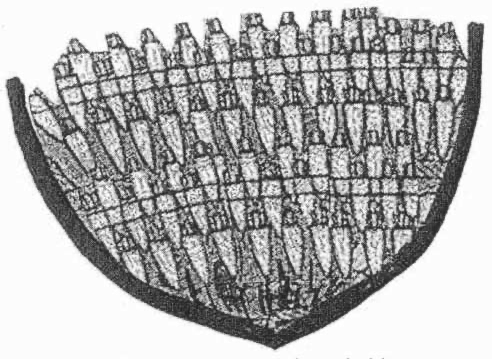
\includegraphics[width=.8\textwidth]{amphora_stowage_aboard_ship.png}
    \end{center}
    \caption{The egg-like shape enabled amphoras to interlock and minimize the waste of space on a ship.
    Source: \cite{twede2002commercial}.}
  \end{figure}

  Amphoras' various shapes and markings - which changed by time, region, producer, contents, and brand
  identity - were used to identify the package status and the different products inside \cite{twede2002commercial}.

  \begin{figure}[ht]
    \begin{center}
      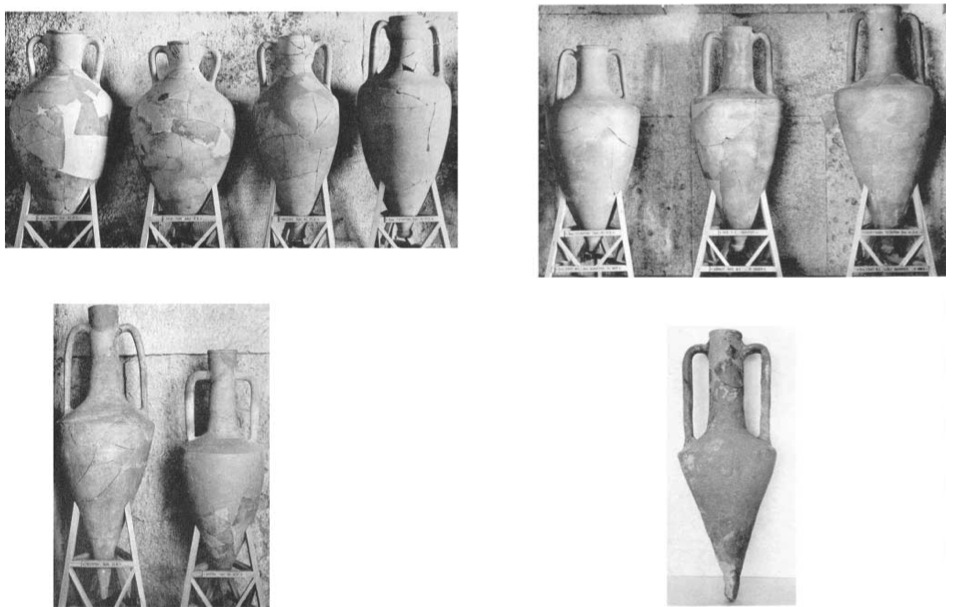
\includegraphics[width=.8\textwidth]{amphora_various_shape.png}
    \end{center}
    \caption{Amphoras have various shapes. Source: \cite{twede2002commercial}.}
  \end{figure}

  Amphoras have great significance in archaeology. They can be used as evidence for the trade patterns throughout
  the Mediterranean \cite{twede2002commercial}. As they were usually discarded at the destination of a trade and have been
  found in shipwrecks, archaeologists have been using them to recreate the transit routes \cite{twede2002commercial}.
  Furthermore, researchers have been able to classify different amphoras, which also helps to date ruins and shipwrecks
  \cite{twede2002commercial}.

  \subsubsection{Computer Vision for Underwater Archaeology}

  Computer vision is the science of perceiving and understanding the world through images and videos \cite{elgendy2020deep}.
  There have been multiple exciting applications of computer vision, including image classification \cite{rawat2017deep},
  object detection and localization \cite{zhao2019object,liu2020deep}, art generation (neural style transfer)
  \cite{jing2019neural}, image creation with Generative Artificial Networks (GAN) \cite{goodfellow2014generative},
  face recognition \cite{parkhi2015deep}, action and activity recognition \cite{poppe2010survey}, human pose estimation
  \cite{toshev2014deeppose}, and image recommendation system \cite{niu2018neural}.

  However, there is still limited research for the application of computer vision and machine learning in archaeology,
  especially underwater archaeology, compared to other domains \cite{maaten2007computer, qin2015underwater}.
  Computer vision, instead of visual inspection, could be used to automate the detection, assessment, and classification
  of artifacts \cite{maaten2007computer}.

  Underwater computer vision has proven to be challenging, largely due to: 1) the distortion and attenuation caused by
  light propagation in water, and 2) the unrestricted natural environment with the abundance of marine life and suspended
  particles \cite{qin2015underwater, rizzini2015investigation, lu2017underwater}.

  Despite the challenges, computer vision has lower cost \cite{rizzini2015investigation} compared to sonar imagery
  \cite{abu2019statistically} and laser scanning \cite{gordon1992use}. Plus, the increasingly abundant visual data obtained
  through autonomous underwater vehicles (AUVs), unmanned underwater vehicles (UUVs)
  \cite{lu2017underwater, moniruzzaman2017deep}, and seafloor cabled observatories \cite{qin2015underwater} enables us
  to utilize deep learning.

  Furthermore, the research for deep-water shipwrecks is even more limited, mostly due to the lack of information and
  accessibility \cite{drap2015underwater}. However, the need to study deep-water sites are in high demand, as the threats
  to these sites are increasing \cite{drap2015underwater}. One major threat is the new forms of trawling that destroy the
  surface of these sites and interfere with the readability \cite{drap2015underwater}. This means that many
  shipwrecks are likely to be damaged before they can be studied \cite{drap2015underwater}. It is thus crucial to implement
  efficient, accessible, and accurate techniques like deep learning based computer vision to study deep-water shipwrecks.

  \subsection{Deep Learning}

  Machine learning is the class of algorithms that allow computers to learn and improve from data instead of being
  explicitly programmed \cite{samuel1959some, geron2019hands}. And deep learning is the subfield of machine learning that
  builds artificial neural networks with more than one layer between the input and output layers
  \cite{geron2019hands, burkov2019hundred, zhang2018definition}. Deep learning constructs complex representations by
  combining simpler ones from the previous layers \cite{goodfellow2016deep}.

  \begin{figure}[ht]
    \begin{center}
      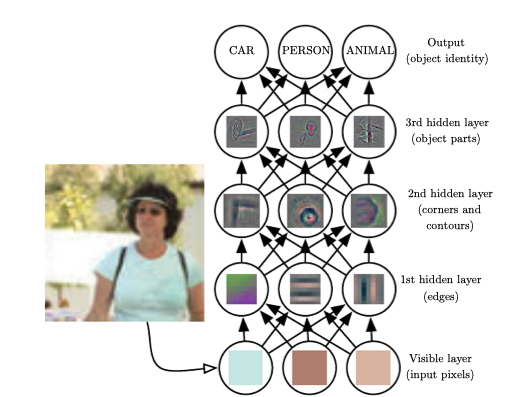
\includegraphics[width=.8\textwidth]{deep_learning.png}
    \end{center}
    \caption{A deep learning system that learns the representations of a person. This is achieved by combining simpler
    features like corners and contours, which are further expressed by combining simpler features like edges. Source:
    \cite{goodfellow2016deep}}
  \end{figure}

  \subsubsection{Artifical Neural Networks (ANNs)}

  Inspired by the biological neuron, artificial neural networks (ANNs) were first introduced in 1943 using propositional
  logic \cite{mcculloch1943logical}. The artificial neuron activates its single binary output when the number of active
  binary inputs reaches the activation threshold, which enables us to build networks that can perform any logical
  computation \cite{geron2019hands, mcculloch1943logical}.

  \begin{figure}[ht]
    \begin{center}
      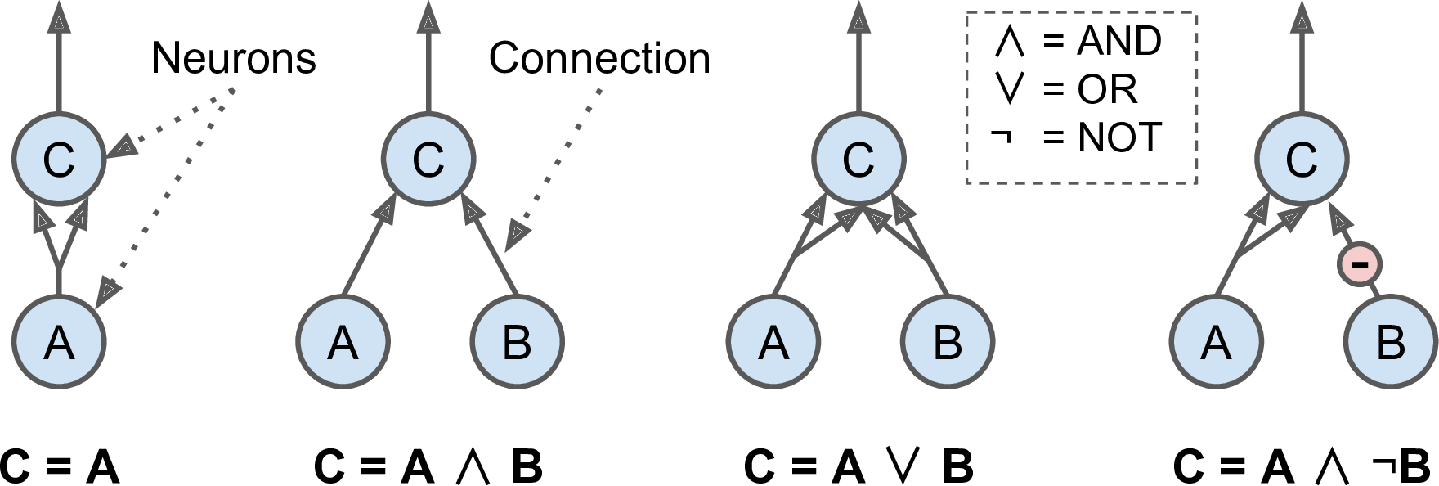
\includegraphics[width=.8\textwidth]{ann_logic_computations.png}
    \end{center}
    \caption{ANNs performing logical computations with the activation threshold of 2. Source: \cite{geron2019hands}}
  \end{figure}

  Then the Perceptron was introduced in 1957, which is based on a different artificial neuron called threshold logic unit
  (TLU) or linear threshold unit (LTU) \cite{rosenblatt1957perceptron}. The inputs and outputs are numbers instead of
  binary values, and each input has a weight. TLU computes the weighted sum of the inputs and then applies a step
  function like the Heaviside function
  $heaviside (x) =
  \begin{cases}
    0 & x \le 0 \\
    1 & x \geq 0 \\
  \end{cases}$
  \cite{geron2019hands, rosenblatt1957perceptron}.

  \begin{figure}[ht]
    \begin{center}
      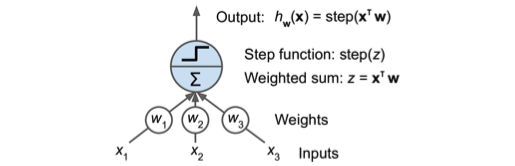
\includegraphics[width=.8\textwidth]{tlu.png}
    \end{center}
    \caption{Threshold logic unit. Source: \cite{geron2019hands}}
  \end{figure}

  A single TLU can be used for simple linear binary classification, while a layer of TLUs plus a bias neuron form a
  Perceptron capable of multi-output classification \cite{geron2019hands}.

  \begin{figure}[ht]
    \begin{center}
      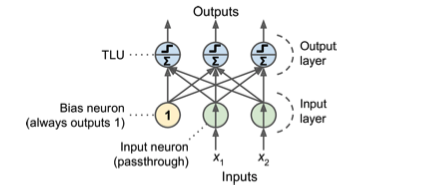
\includegraphics[width=.8\textwidth]{perceptron.png}
    \end{center}
    \caption{A Perceptron with three output neurons. Source: \cite{geron2019hands}}
  \end{figure}

  The outputs of a fully connected layer is computed as follows, where $\mathbf{X}, \mathbf{W}, \mathbf{b}$, and $\phi$
  are respectively the input matrix, weight matrix, bias vector, and activation function:

  $$h_{\mathbf{W,b}}(\mathbf{X}) = \phi(\mathbf{XW} + \mathbf{b})$$

  The Perceptron is trained using a variant of the Herbb's rule \cite{hebb2005organization}, which is famously summarized
  as "neurons wire together if they fire together \cite{lowel1992selection}" \cite{geron2019hands}. However, the Perceptron
  can not learn complex patterns due the linear decision boundary of the output neurons, and it can only make predictions
  based on a hard threshold instead of outputting a class probability \cite{geron2019hands}. To address these limitations,
  the Multilayer Perceptron (MLP) was introduced by stacking multiple Perceptrons.

  \begin{figure}[ht]
    \begin{center}
      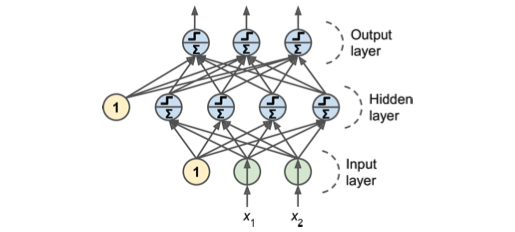
\includegraphics[width=.8\textwidth]{mlp.png}
    \end{center}
    \caption{A Multilayer Perceptron with one hidden layer. Source: \cite{geron2019hands}}
  \end{figure}

  Backpropagation \cite{rumelhart1985learning} is used to train the MLP, which first makes a prediction and measures the
  error in the forward pass, then measures the error contribution from each connection in the reverse pass, and finally
  tweaks the connection weights to reduce teh error in the Gradient Descent \cite{ruder2016overview} step
  \cite{geron2019hands}. Activation functions like Rectified Linear Unit $ReLU(x) = max(0, x)$ are used to add
  nonlinearity, which theoretically gives a large enough deep neural network the ability to approximate any continuos
  function \cite{geron2019hands}.

  \subsubsection{Convolutional Neural Networks (CNNs)}

  Convolutional Neural Networks (CNNs) were inspired by the brain's visual cortex, and they have been used in computer
  vision since the 1980s \cite{geron2019hands}. We can not simply use a deep neural network with fully connected layers
  for computer vision, as it breaks down for large images due to the huge number of parameters it requires
  \cite{geron2019hands}. CNNs also have successful applications in other domains like recommender systems
  \cite{van2013deep} and natural language processing (NLP) \cite{collobert2008unified}.

  Hubel et al. \cite{hubel1959single, hubel1959receptive, hubel1968receptive} found that many biological neurons have
  a small receptive field, which  means they only react to visual stimuli in a limited region of the visual field
  \cite{geron2019hands}. Some neurons only react to horizontal lines, while others only react to lines with
  different orientations \cite{geron2019hands}. Some neurons have larger receptive fields, and they react to more complex
  patterns formed by lower-level patterns \cite{geron2019hands}.

  Neurons in the first convolutional layer are only connected to pixels in their receptive fields, and neurons in the
  second convolutional layer are only connected to the neurons in a small receptive field in the first layer
  \cite{geron2019hands}. This allows the CNN to concentrate on lower-level features in the first hidden layer, then
  combine them into higher-level features in the second hidden layer, and so on \cite{geron2019hands}.

  \begin{figure}[ht]
    \begin{center}
      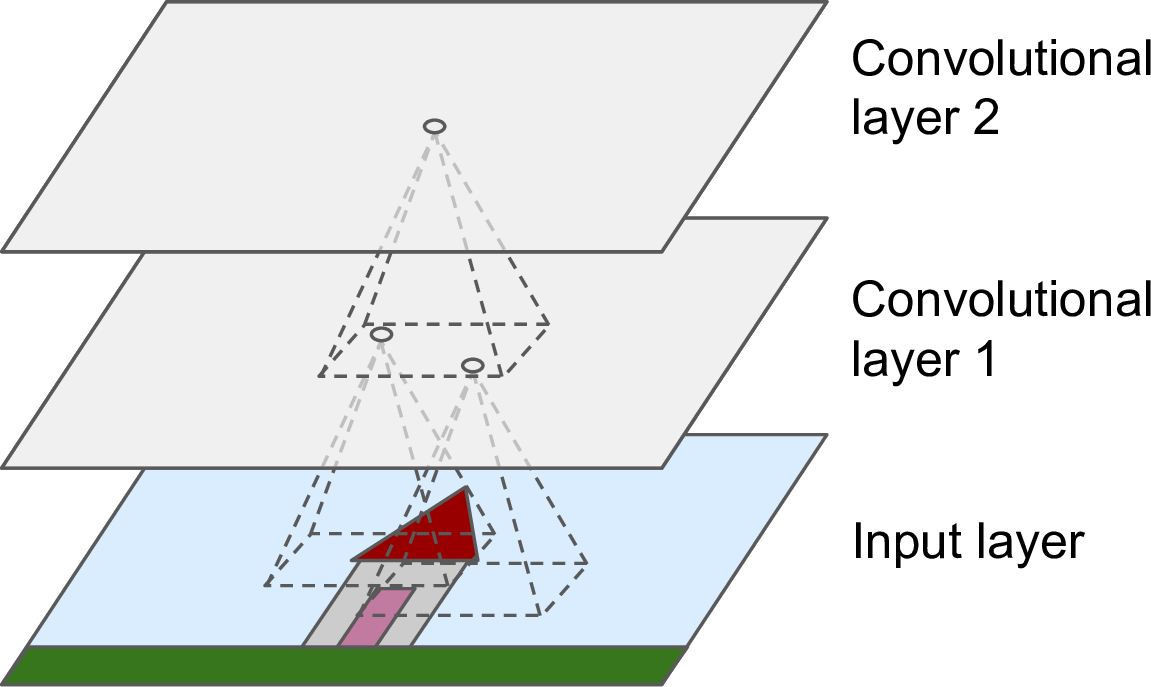
\includegraphics[width=.8\textwidth]{cnn_layers.png}
    \end{center}
    \caption{CNN layers with rectangular receptive fields. Source: \cite{geron2019hands}}
  \end{figure}

  The filters or convolution kernels, which are learned during training, are neurons' weights that can be presented as
  small images the size of receptive fields \cite{geron2019hands}. For example, a black sqaure with a horizontal white
  line in the middle (a matrix full of 0s except for the central row with 1s) is a filter that only reacts to the central
  row in the receptive field. A layer of neurons with the same filter outputs a feature map, which highlights the parts
  of an image that activate the filter the most \cite{geron2019hands}.

  \begin{figure}[ht]
    \begin{center}
      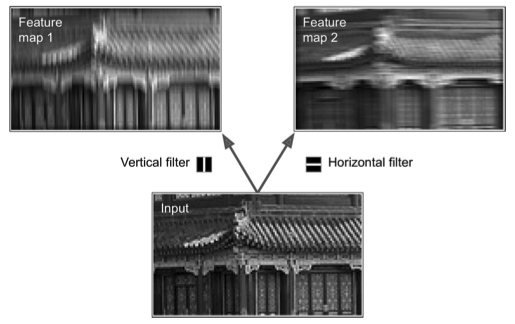
\includegraphics[width=.8\textwidth]{filters.png}
    \end{center}
    \caption{Two feature maps obtained by applying two different filters. Source: \cite{geron2019hands}}
  \end{figure}

  The pooling layers subsample (i.e. shrink) the input image to reduce the computational load and the number of paramters,
  which also reduces overfitting \cite{geron2019hands}. Plus, pool layers can bring some invariance to small translations,
  rotations, and scaling \cite{geron2019hands}.

  \begin{figure}[ht]
    \begin{center}
      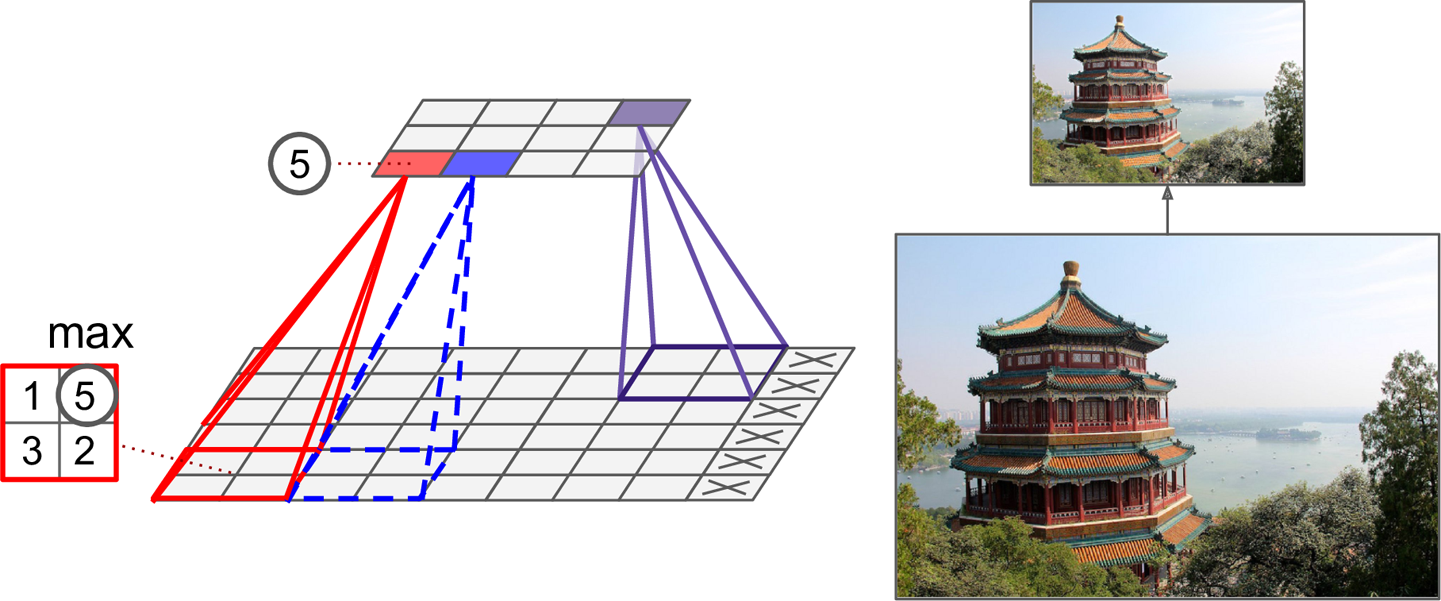
\includegraphics[width=.8\textwidth]{max_pooling.png}
    \end{center}
    \caption{A max pooling layer with a 2 x 2 kernel and stride 2. Only the max value from each receptive field
    gets passed to the next layer. Source: \cite{geron2019hands}}
  \end{figure}

  \begin{figure}[ht]
    \begin{center}
      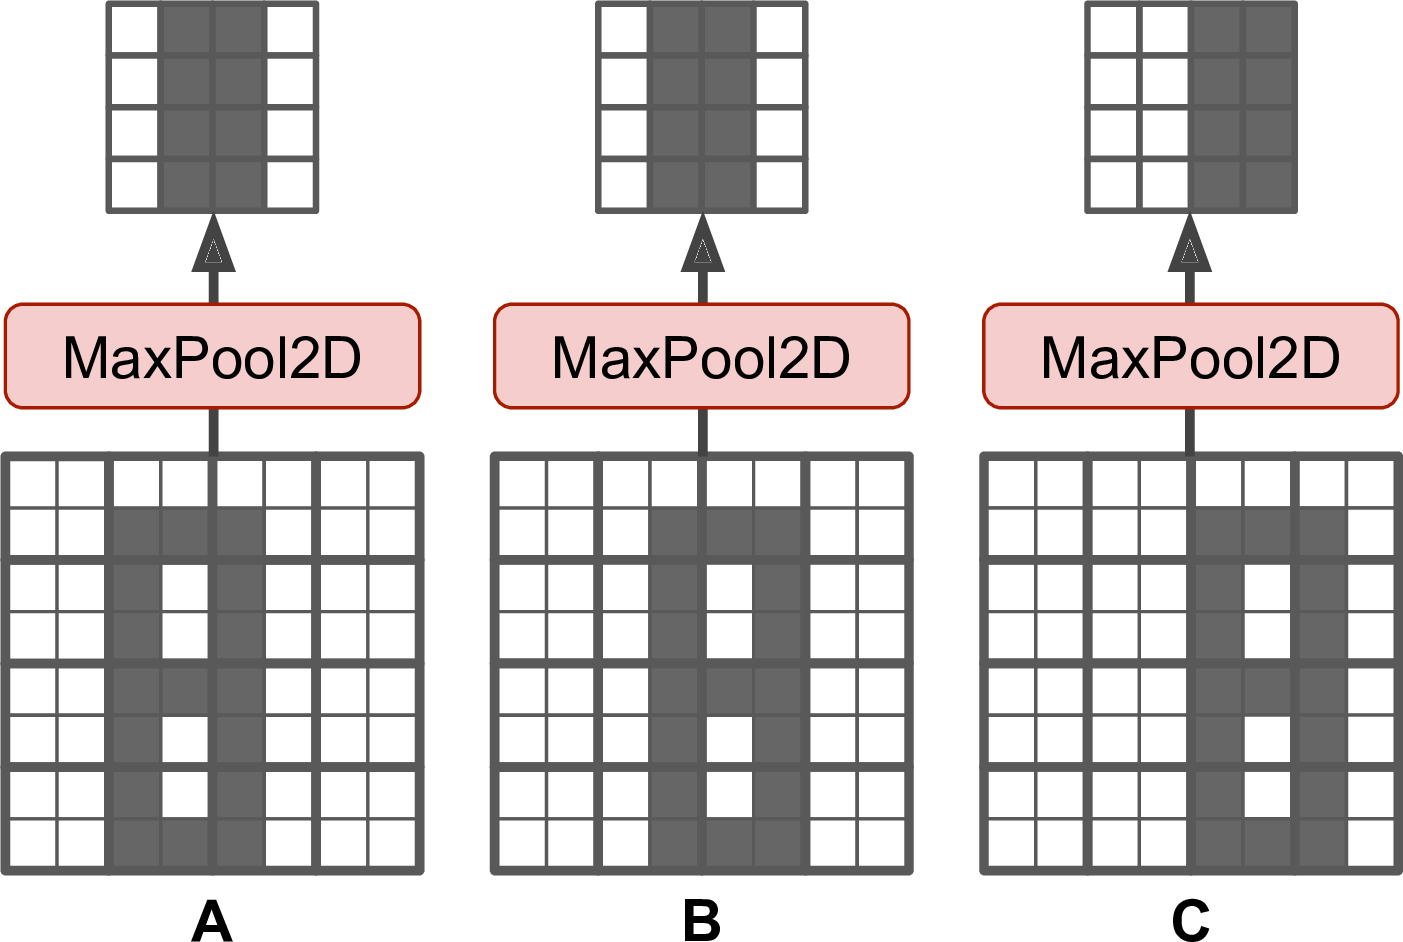
\includegraphics[width=.8\textwidth]{max_pooling_invariance.png}
    \end{center}
    \caption{Max pooling layer's invariance to small translations. Source: \cite{geron2019hands}}
  \end{figure}

  The typical CNN architecture involves the aforementioned convolutional layers, pooling layers, and fully connected layers.
  Some well-established CNN architecutres are LeNet-5 \cite{lecun1998gradient}, AlexNet \cite{krizhevsky2012imagenet},
  GoogLeNet \cite{szegedy2015going}, VGGNet \cite{simonyan2014very}, ResNet (Residual Network) \cite{he2016deep}, Xception
  (Extreme Inception) \cite{chollet2017xception}, and SENet (Squeeze-and-Excitation Network) \cite{hu2018squeeze}.

  \begin{figure}[ht]
    \begin{center}
      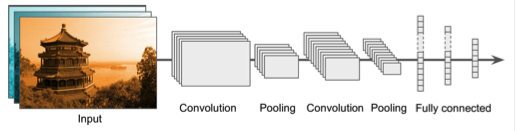
\includegraphics[width=.8\textwidth]{typical_cnn.png}
    \end{center}
    \caption{The typical CNN architecuture. Source: \cite{geron2019hands}}
  \end{figure}

  Here we give ResNet a more in-depth introduction, as it's the backbone network in the model we use to detect amphoras.
  ResNet is a fully convolutional network (FCN) \cite{he2016deep, long2015fully}. FCNs contain only convolutional layers
  and pooling layers, which means input images can have arbitrary sizes \cite{long2015fully}. Resnet adds skip connections
  (or shortcut connections), which means the input signal of a layer is also added to the ouput of a higher up layer
  \cite{geron2019hands, he2016deep}. Skip connections help speed up the training considerably, since: 1) the network
  preconditions the problem to be the identify function, which is often close to the target function, and 2) the network
  can start making progress even if some layers have not started learning yet \cite{geron2019hands, he2016deep}.

  \begin{figure}[ht]
    \begin{center}
      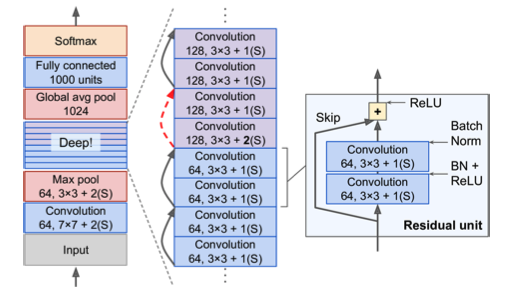
\includegraphics[width=.8\textwidth]{resnet.png}
    \end{center}
    \caption{ResNet architecture. Source: \cite{geron2019hands}}
  \end{figure}

  \subsubsection{Deep Learning vs. Traditional Computer Vision}

  \subsection{Object Detection}

  Define object detection and introduce the sliding CNN approach.

  \subsubsection{Fully Convolutional Networks (FCNs)}

  \subsubsection{General Object Detection Framework Components}

  \paragraph{Region Proposals}
  \paragraph{Network Predictions}
  \paragraph{Non-Maximum Suppression (NMS)}
  \paragraph{Metrics}

  \subsubsection{Region-Based Convultional Neural Networks (R-CNN)}

  \paragraph{R-CNN}
  \paragraph{Faster R-CNN}
  \paragraph{Faster R-CNN}

  \subsubsection{Single Shot Detector (SSD)}
  \subsubsection{You Only Look Once (YOLO)}

  \paragraph{YOLO}
  \paragraph{YOLOv2}
  \paragraph{YOLOv3}
  \paragraph{YOLOv4}
  \paragraph{YOLOv5}

  \section{Related Work}
  % \cite{moniruzzaman2017deep, qin2015underwater, pasquet2017amphora, mccarthy20193d}


  \section{Data and Methods}

  This is the technical core of the thesis. Here you lay out your how
  you answered your research question, you specify your design of
  experiments or simulations, point out difficulties that you
  encountered, etc.

  (target size: 5-10 pages)

  \subsection{Data}
  \subsection{Model}
  \subsection{Model Training}

  \section{Evaluation}

  This section discusses criteria that are used to evaluate the
  research results. Make sure your results can be used to published
  research results, i.e., to the already known state-of-the-art.

  (target size: 5-10 pages)

  \begin{table}[ht]
    \begin{center}
      \begin{tabular}{cl}
        \toprule
        Number & Description \\
        \midrule
        7 & A lucky number in Western culture \\
        8 & A lucky number in Chinese and other Asian cultures \\
        42 & Answer to the ultimate question of life, the universe, and everything \\
        404 & Not found \\
        \bottomrule
      \end{tabular}
      \caption{Useless insights I gained with no further meaning}
    \end{center}
  \end{table}

  \subsection{Visual Evaluation}
  \subsection{Metric Evaluation}

  \section{Conclusions}

  Summarize the main aspects and results of the research
  project. Provide an answer to the research questions stated earlier.

  (target size: 1/2 page)

  \section{Future Work}

  \newpage

  \printbibliography

\end{document}
